\chapter{Algoritmos de clustering con restricciones}\label{ch:Algoritmos}

Una vez introducido el problema del clustering con restricciones, pasamos a profundizar en los métodos para su aplicación. La siguiente sección presenta 5 algoritmos de clustering con restricciones, cuyos resultados serán expuestos más tarde, en la Sección \ref{ch:Experimentación}.

\section{Formalización del problema}

Definido ya el problema del clustering con restricciones en la Sección \ref{ch:Clustering con restricciones}, especificamos la manera de notar sus elementos, de forma que sea sencillo referirse a ellos.

\begin{itemize}
	
	\item Notaremos con $X$ a la matriz de $n\times p$ que contiene el conjunto de datos de entrada.
	
	\item Notaremos con $x_i \;\; t.q. \;\; i \in \{1, \cdots, n\}$ a cada instancia de $X$, por lo que $x_i$ es un vector en el espacio $\mathbb{R}^p$ ($x_i \in \mathbb{R}^p$).
	
	\item Notaremos con $R$ al conjunto de restricciones, tanto las de tipo \acs{ML} como las \acs{CL}, es decir $R = ML \cup CL$. 
	
	\item Notaremos con $K$ el número de clusters de la partición resultante.
	
	\item Notaremos con $C$ el conjunto de clusters, y con $c_i \; t.q. \; i \in \{1, \cdots, K\}$ a cada uno de ellos, por tanto $C = \{c_i, \cdots, c_K\}$.
	
	\item Notaremos con $V$ la matriz de $K\times p$ que almacena el conjunto de centroides asociados a los clusters, de manera que $v_i \in \mathbb{R}^p$ corresponde al cluster $c_i$.
	
\end{itemize}
Cabe destacar que los elementos y parámetros particulares de cada algoritmo serán definidos en la sección correspondiente al mismo, así como que no todos los elementos expuestos anteriormente son comunes a todos los algoritmos; si bien sí que lo son a la mayoría de ellos.

\section{COP-K-means (Constrained K-means)} \label{copkm}

El algoritmo K-medias (\acs{KM}, Apéndice \ref{ap:kmeans}) es uno de los más básicos para aplicar clustering. Así, el algoritmo COP-K-medias (\textit{COP-K-means}) es la adaptación inmediata de \acs{KM} al clustering con restricciones. Para realizar un estudio detallado sobre el mismo tomaremos como base el trabajo de Wagstaff et al. (2001) \cite{Wagstaff:2001b}.

El cambio más notable que supone COP-K-medias respecto al tradicional K-medias, consiste en modificar la regla de asignación de instancias a clusters de este último, para comprobar que dicha asignación no viola ninguna restricción. De esta manera, en cada iteración se intenta asignar cada instancia $x_i$ al cluster más cercano $c_j$. Esta asignación sólo se llevará a cabo si, como hemos dicho, no se viola ninguna restricción. Si existe una instancia $x_{ML}$ que debe ser asignada al mismo cluster que $x_i$, pero ya ha sido incluida en otro cluster, o existe una instancia $x_{CL}$ en $c_j$ que no puede ser agrupada junto a $x_i$, entonces $x_i$ no puede ser asignado a $c_j$. El proceso continúa hasta encontrar una asignación legal para $x_i$, en caso de que no se encuentre se devuelve la partición vacía como resultado. Así el algoritmo proporciona una partición de $X$ que cumple necesariamente todas las restricciones especificadas en $R$. El Algoritmo \ref{alg:ckm} corresponde al pseudocódigo asociado a COP-K-medias \cite{Wagstaff:2001b}:


\begin{algorithm}
	
	\BlankLine
	\KwIn{Conjunto de datos $X$, conjunto de restricciones $R$, número de clusters $K$.}
	\KwOut{Partición $P$ del conjunto de datos $X$.}
	\BlankLine
	\textbf{función} COP-K-medias($X$, $R$, $K$) \Begin{
		\BlankLine
		1. Sean $V = \{v_1,\cdots ,v_K\}$ los centroides iniciales\\
		2. Asignar cada instancia $x_i \in X$, al cluster $c_j$ asociado al centroide más cercano $v_j$ tal que ViolaRestriccion($x_i$, $c_j$, $R$) = falso. Si no existe $c \in C \;\;\; t.q.$ ViolaRestriccion($x_i$, $c_j$, $R$) = falso, \KwRet $\emptyset$.\\
		3. Para cada cluster $c_i$, actualizar su centroide $v_i$ realizando un promedio de todas las instancias $x_i$ asignadas a él.\\
		4. Iterar entre (1.) y (2.) hasta converger.\\
		5. \KwRet $C$
		\BlankLine
	}
	\BlankLine
	\KwIn{Instancia $x$, cluster $c$, conjunto de restricciones $R$}
	\BlankLine
	\textbf{función} ViolaRestriccion($x$, $c$, $R$) \Begin{
		\BlankLine
		1. Para cada $(x, x_{ML}) \in ML$, si $x_{ML} \notin R$ \KwRet \textbf{true}.\\
		2. Para cada $(x, x_{CL}) \in CL$, si $x_{CL} \notin R$ \KwRet \textbf{true}.\\
		3. En otro caso, \KwRet \textbf{false}.
		\BlankLine
	}
	
	\caption{COP-K-medias}\label{alg:ckm}
\end{algorithm}

Existen multitud de criterios de convergencia estandarizados, aunque es común emplear uno adaptado al problema particular que queramos solucionar. El más extendido consiste en calcular la diferencia de la posición de los centroides entre dos iteraciones sucesivas, de forma que cuando ésta sea menor que un umbral dado detenemos el proceso de iteración.

\section{CEKM (Constrained Evidential K-means)} \label{cekm}

Tal y como indican Violaine et al. (2012) \cite{CECM:2012}, cuyo trabajo es el fundamento de la siguiente sección, para comprender el algoritmo  \acf{CEKM}, primero es necesario realizar una introducción al algoritmo K-medias difuso (\textit{Fuzzy K-means}, \acs{FKM}). En él, cada instancia puede pertenecer a uno o más clusters, con diferentes grados de pertenencia. La matriz que almacena esta información, es decir, la partición difusa, se nota con $U$, y se calcula minimizando la siguiente función:

\begin{equation}
\sum_{j=1}^{K} u_{ij} \;\; t.q. \;\; u_{ij} \in [0,1] \forall i,j
\label{eqn2}
\end{equation}

Donde $u_{ij}$ representa el grado de pertenencia de la instancia $i$ al cluster $j$, y $K$ es el número de clusters. Sin embargo, este método puede producir resultados contraintuitivos cuando los datos a los que se aplica son ruidosos o presentan instancias aisladas (\textit{outliers}).

El clustering evidencial (\textit{evidential clustering}) da solución a los problemas que presenta el algoritmo \acs{FKM}, introduciendo el concepto de partición de creencia (\textit{credal partition}), que extiende los conceptos existentes de particiones fuertes, difusas y probabilísticas. De esta forma, en una partición de creencia, se asigna a cada instancia una masa de creencia (\textit{mass of belief}), no sólo para un único cluster, sino para cualquier conjunto de los mismos. El método \acs{CEKM} combina las ventajas del uso de las restricciones con las del uso de funciones de creencia.

\subsection{Funciones de creencia}

La teoría de la evidencia de Dempster-Shafer ofrece un marco teórico para trabajar con información parcial y no completamente fiable; tomamos de ella los conceptos relativos a las funciones de creencia.

Consideremos la variable $c$ que toma valores en el conjunto finito $C = \{c_1 \cdots c_K \}$. El conocimiento parcial sujeto al valor real que adopta $c$ puede ser representado mediante una función de masa $m$, que es una aplicación de $C$ al intervalo $[0,1]$:

\begin{equation}
\sum_{A \subseteq C} m(A) = 1
\label{eqn3}
\end{equation}

A los subconjuntos $A$ de $C$ que cumplen que $m(A) > 0$ se los denomina conjuntos focales (\textit{focal sets}) de $m$. El valor del conjunto focal $m(A)$ se interpreta como la fracción de una unidad de masa de creencia que está asignada a $A$ y que no puede ser asignada a ningún otro subconjunto de $A$. Si el único conjunto focal es $C$, nos encontramos en el caso de completa ignorancia sobre los datos. Por el contrario, si la masa de creencia se asigna a un único elemento de $C$, estaríamos en el caso de certeza absoluta.

Se dice que una función de masa $m$ está normalizada si $m(\emptyset) = 0$. Sin embargo, bajo la hipótesis de mundo abierto, una función de masa en la que $m(\emptyset) > 0$ se interpreta como la cantidad de creencia que se le asigna a la hipótesis de que el verdadero valor de $c$ puede no encontrarse en $C$.

Dada una función de masa $m$, podemos definir una función de plausibilidad $pl:2^C \rightarrow [0,1]$ y una función de creencia $bel: 2^C \rightarrow [0,1]$ de la siguiente manera:

\begin{equation}
pl(A) = \sum_{B \cap A \neq \emptyset} m(B) \;\;\; \forall A \subseteq C
\label{eqn4}
\end{equation}

y 

\begin{equation}
bel(A) = \sum_{B \subseteq A, B \neq \emptyset} m(B) \;\;\; \forall A \subseteq C
\label{eqn5}
\end{equation}

De esta forma, las funciones $pl$ y $bel$ están relacionadas como sigue:

\begin{equation}
pl(A) = 1 - m(\emptyset) - bel(\bar{A})
\label{eqn6}
\end{equation}

Donde $\bar{A}$ representa el complemento de $A$.  La cantidad $bel(A)$ se interpreta como el grado de creencia en $A$, tomando en consideración la masa de creencia asignada a $A$ y a los subconjuntos no vacíos de $A$. Por el contrario, $pl(A)$ mide hasta qué punto es erróneo no creer en $\bar{A}$.

Con el objetivo de tomar decisiones en base al valor de $c$, es posible transformar la función de masa en una distribución de probabilidad pignística, definida, para una función de masa normalizada, como:

\begin{equation}
BetP(c) = \sum_{c \in A} \frac{m(A)}{|A|} \;\;\; \forall c \in C
\label{eqn7}
\end{equation}

\subsection{FKM (fuzzy K-means) y sus variantes}

Cada cluster $c_j \in C$ con $j \in \{1,\cdots,K\}$ está representado por un vector $v_j \in \mathbb{R}^p$, esto es, un centroide. Además, definimos $V$ como la matriz compuesta por todos los centroides, y $U = (u_{ij})$ como la partición difusa que contiene los grados de pertenencia de cada instancia de $X$ a cada cluster. El algoritmo \acf{FKM} calcula las matrices $U$ y $V$ de manera que minimiza (sujeto a las Ecuaciones \ref{eqn2} y \ref{eqn3}) la siguiente función:

\begin{equation}
J_{FKM}(U,V) = \sum_{i=1}^{n}\sum_{j=i}^{K} u_{ij}^\beta d_{ij}^2
\label{eqn8}
\end{equation}

Donde $d_{ij}$ representa la distancia Euclídea entre el objeto $x_i$ y el centroide $v_j$, y donde $\beta > 1$ es el exponente que controla el grado de difusión de la partición. La función objetivo se minimiza mediante un algoritmo iterativo que optimiza los centroides y los grados de pertenencia de manera alterna. El algoritmo empieza con una asignación inicial sobre la que realiza modificaciones hasta que converge.

Para detectar datos ruidosos u outliers empleamos el algoritmo \acs{NC} \textit{Noise-Clustering}. Este método consiste en añadir a los $K$ clusters iniciales uno adicional llamado ``cluster ruidoso'', asociado a una distancia fija $\rho$ respecto a todos los objetos. El parámetro $\rho$ controla la cantidad de datos que serán considerados como outliers. La pertenencia $u_{i*}$ de un objeto $i$ al cluster ruidoso se calcula como:

\begin{equation}
u_{i*} = 1 - \sum_{j=1}^{K} u_{i,j} \;\;\; i = {1,\cdots,n}
\label{eqn9}
\end{equation}

Por tanto, la función objetivo que minimiza el algoritmo \acs{NC} no es más que una combinación del cálculo de pertenencia de objetos al cluster ruidoso y de la que minimizaba el algoritmo \acs{FKM}:

\begin{equation}
J_{NC}(U,V) = \sum_{i=1}^{n}\sum_{j=i}^{K} u_{ij}^\beta d_{ij}^2 + \sum_{i=1}^{K} \rho^2 u_{i*}^\beta
\label{eqn10}
\end{equation}

\subsection{El algoritmo EKM (Evidential K-means)}

Es posible obtener una versión credibilística del algoritmo \acs{NC} reemplazando la matriz asociada a la partición difusa $U$ con una partición de creencia, que notaremos con $M$. En este contexto, el conocimiento parcial asociado a la pertenencia de un objeto a una clase viene representado por una función de masa aplicada al conjunto $C$ de posibles clases. Por tanto, la masa de creencia puede ser asignada a cualquier subconjunto $A$ de $C$, y no sólo a elementos únicos de $C$. Este esquema hace posible modelar una amplia variedad de circunstancias, que van de la completa ignorancia sobre el conjunto de datos hasta la completa certeza sobre el mismo.

Para ilustrar estas ideas se propone el siguiente ejemplo: consideramos un conjunto de cuatro objetos que deben ser clasificados en dos clases. La Tabla \ref{tab:tabla2} contiene la partición de creencia asociada a estos datos. La clase del primer objeto es conocida con certeza, ya que su masa de creencia está asignada a un solo elemento de $C$. Por el contrario, la clase del segundo objeto es completamente desconocida. La masa de creencia del tercer objeto está repartida entre dos elementos de $C$. Por tanto, tenemos conocimiento probabilístico sobre la clase a la que pertenece. El último objeto representa un outlier, ya que su masa de creencia está asignada al conjunto vacío.

\begin{table}[h]
	\centering
	\setlength{\arrayrulewidth}{1mm}
	\setlength{\tabcolsep}{10pt}
	\renewcommand{\arraystretch}{1}
	
	\rowcolors{2}{gray!25}{white}
	\begin{tabular}{ >{\centering\arraybackslash}m{1cm}  >{\centering\arraybackslash}m{1cm}>{\centering\arraybackslash}m{1cm}>{\centering\arraybackslash}m{1cm}>{\centering\arraybackslash}m{1cm}}
		\hline
		\rowcolor{black}
		\multicolumn{5}{c}{\bf \color{white}{Ejemplo de partición de creencia}}\\
		\hline
		\rowcolor{gray!50}
		\textbf{$A$} & \textbf{$m_1(A)$} & \textbf{$m_2(A)$} & \textbf{$m_3(A)$} & \textbf{$m_4(A)$} \\
		$\emptyset$ & $0$ & $0$ & $0$ & $1$ \\
		$\{c_1\}$ & $1$ & $0$ & $0.3$ & $0$ \\
		$\{c_2\}$ & $0$ & $0$ & $0.7$ & $0$ \\
		$C$ & $0$ & $1$ & $0$ & $0$ \\
		\hline
		
	\end{tabular}
	\caption[Ejemplo de partición de creencia]{Ejemplo de partición de creencia \cite{CECM:2012}}
	\label{tab:tabla2}
\end{table}

\acf{EKM} es uno de los algoritmos que opera con una partición de creencia obtenida en base a los datos. Si tomamos $m_{ij}$ como el grado de creencia de que el objeto $x_i$ pertenece al subconjunto $A_j \subseteq C$, obtener una partición de creencia implica determinar, para cada $x_i$, las cantidades $m_{ij} = m_i(A_j)\;\; \forall A_j \neq \emptyset, A_j \subseteq C$. De esta manera, cuando la distancia $d_{ij}$ entre $x_i$ y $A_j$ es alta (baja), $m_{ij}$ será un valor bajo (alto).

Tal y como sucedía en \acf{FKM}, cada clase $c_l$ está representada por un centroide $v_l \in \mathbb{R}^p$. Entonces, para cada subconjunto $A_j$ de $C$ distinto de $\emptyset$ se calcula su centroide $\bar{v}_j$ como el baricentro de los centros asociados a las clases presentes en $A_j$:

\begin{equation}
\bar{v}_j = \frac{1}{|A_j|} \sum_{l=1}^{K} S_{lj} v_l
\label{eqn11}
\end{equation}

donde el valor $S_{lj}$ viene definido por:

\begin{equation}
S_{lj} = \begin{cases}
1 \;\;\; \textbf{si} \;\;\; c_l \in A_j\\
0 \;\;\; \textbf{otro caso}
\end{cases}
\label{eqn12}
\end{equation}

La distancia $d_{ij}$ entre la instancia $x_i$ y el conjunto focal $A_j$ se calcula como:

\begin{equation}
d_{ij} = ||x_i - \bar{v}_j||
\label{eqn13}
\end{equation}

Entonces, el algoritmo \acs{EKM} calcula las matrices $M$ y $V$ tratando de minimizar un criterio similar al del algoritmo \acs{NC}:

\begin{equation}
J_{EKM}(M,V) = \frac{1}{2^cn} \sum_{i=1}^{n}\sum_{A_j \neq \emptyset} |A_j|^\alpha m_{ij}^\beta d_{ij}^2 + \sum_{i=1}^{n} \rho^2 m_{i\emptyset}^\beta
\label{eqn14}
\end{equation}

sujeto a las restricciones $m_{ij} \ge 0 \;\; \forall i,j$, y $m_{i\emptyset} \ge 0 \;\; \forall i$, y:

\begin{equation}
\sum_{j/A_j \subseteq C, A_j \neq \emptyset} m_{ij} + m_{i\emptyset} = 1 \;\;\; \forall i = 1,n
\label{eqn15}
\end{equation}

Donde $m_{i\emptyset}$ denota la cantidad de masa de creencia de la instancia $x_i$ asignada al conjunto vacío. El parámetro $\rho$ representa la distancia de cualquier objeto al conjunto vacío, y el parámetro $\alpha$ se introduce para controlar la penalización por asignar objetos a conjuntos con alta cardinalidad.

Gracias a la restricción expuesta en la Ecuación \ref{eqn15}, podemos obtener equivalencia entre los algoritmos \acs{NC} y \acs{EKM}. El algoritmo \acs{EKM} asigna una gran masa de creencia al conjunto vacío para un objeto dado cuando éste se encuentra lejos de todos los subconjuntos $A_j$.

Como en \acs{FKM} y \acs{NC}, la partición de creencia se calcula aplicando un proceso de optimización iterativo, que actualiza las masas  y los centroides de forma alterna. La regla de optimización de $M$ es muy similar a su homóloga en \acs{NC}, excepto por el número de valores $m_{ij}$ a calcular, que en este caso es $2^c$, en lugar de los $K + 1$ grados de pertenencia que eran necesarios en \acs{NC}. De esta manera, la función de masa queda definida como:

 \begin{equation}
m_{ij} = \frac{|A_j|^{-\alpha/(\beta-1)} d_{ij}^{-2/(\beta-1)}}{\sum_{A_l \ne \emptyset}|A_l|^{-\alpha/(\beta-1)} d_{ij}^{-2/(\beta-1)} + \rho^{-2/(\beta-1)}}
 \label{eqn16}
 \end{equation}
 
 y
 
\begin{equation}
m_{i\emptyset} = 1 - \sum_{A_j \ne \emptyset}m_{ij} \;\;\; i = 1,n
\label{eqn17}
\end{equation}

Por otra parte, la regla de actualización de los centroides resulta un poco más compleja. Requiere resolver un sistema de ecuaciones lineal en cada paso del proceso, en el que cada columna de $V$ es la solución para un sistema lineal de $K$ ecuaciones y $K$ incógnitas. Tomamos $B$ como la matriz de tamaño $(K \times p)$ definida por:

\begin{equation}
B_{lq} = \sum_{i=1}^{n} X_{iq} \sum_{A_j \ni c_l} |A_j|^{\alpha-1} m_{ij}^\beta \;\;\; l = 1,K \;\;\; q =1,p
\label{eqn18}
\end{equation}

y la matriz $H$ de tamaño $(K \times K)$ como:

\begin{equation}
H_{lt} = \sum_{i} \sum_{A_j \supseteq \{c_t,c_l\}} |A_j|^{\alpha - 2} m_{ij}^\beta \;\;\; t,l = 1,K
\label{eqn20}
\end{equation}

de forma que $V$ es la solución del sistema de ecuaciones lineal $H\times V = B$, que puede ser resuelto mediante técnicas estándar.

\subsection{Incorporación de restricciones a EKM}

Una vez definidos los elementos que conforman el algoritmo \acs{EKM}, debemos incorporar las restricciones a nivel de instancia al marco de las funciones de creencia, para integrarlas en el cálculo de la partición de creencia.

Siendo $x_i$ y $x_j$ dos instancias, podemos calcular la función de masa conjunta en el producto cartesiano $C \times C = C^2$ conociendo sus funciones de masa particulares $m_i$ y $m_j$:

\begin{equation}
\begin{split}
m_{i \times j}(A \times B) &= m_i(A)m_j(B) \;\;\; A,B \subseteq C, A \neq \emptyset, B \neq \emptyset\\
m_{i \times j}(\emptyset) & = m_i(\emptyset) + m_j(\emptyset) - m_i(\emptyset)m_j(\emptyset)
\end{split}
\label{eqn21}
\end{equation}

Conociendo $ m_{i \times j} $ es posible calcular la plausibilidad asociada a que los objetos $x_i$ y $x_j$ pertenezcan a la misma clase que, en el espacio $C^2$, corresponde al subconjunto $\theta = \{(c_1, c_1), (c_2, c_2), \cdots, (c_K, c_K)\}$. El caso contrario corresponde al complemento de $\theta$, es decir, $\bar{\theta}$:

\begin{equation}
\begin{split}
pl_{i\times j}(\theta) &= \sum_{A \cap B \ne \emptyset}m_i(A)m_j(B)\\
pl_{i\times j}(\bar{\theta}) &= 1 - m_{i\times j}(\emptyset) - \sum_{l=1}^{K} m_i(\{c_l\})m_j(\{c_l\})
\end{split}
\label{eqn23}
\end{equation}

\subsection{Función objetivo de CEKM}

Asumimos ahora que la partición de creencia es desconocida, y que disponemos del conjunto de restricciones. En tal caso será necesario buscar una partición de creencia que considere las similitudes y diferencias obtenidas en base a los datos y a las restricciones. Para ello debemos buscar que $pl_{i\times j} (\theta)$ sea tan bajo como sea posible si $(x_i, x_i) \in CL$, así como que $pl_{i\times j} (\bar{\theta})$ también lo sea si $(x_i, x_i) \in ML$. A tal fin, integramos una penalización en el criterio de optimización de \acs{EKM} de la siguiente manera:

\begin{equation}
J_{CONST} = \frac{1}{|R|} \left[\sum_{(x_i,x_j) \in ML} pl_{i\times j} (\bar{\theta})\;\; + \sum_{(x_i,x_j) \in CL} pl_{i\times j} (\theta)\right]
\label{eqn25}
\end{equation}

De esta forma, la función objetivo a minimizar pasa a ser:

\begin{equation}
J_{CEKM}(M,V) = (1- \xi)J_{EKM}(M,V) + \xi J_{CONST}
\label{eqn26}
\end{equation}

donde el parámetro $\xi \in [0,1]$ se utiliza para controlar el compromiso entre las restricciones y el modelo geométrico asociado a la métrica de distancia.

\subsection{Proceso de optimización de CEKM}

De igual forma que en \acs{FKM}, \acs{NC} y \acs{EKM}, el modelo de optimización de \acs{CEKM} consiste en actualizar $M$ y $V$ de forma alterna. Cabe destacar que el término de penalización añadido a \acs{CEKM} no depende de los centroides de los clusters, y por tanto se puede aplicar el mismo modelo de actualización que en \acs{EKM} (Ecuaciones \ref{eqn18} y \ref{eqn20}). Generalmente el problema es mucho más complejo para las masas de creencia. Sin embargo, fijando $\beta = 2$, la Ecuación \ref{eqn26}, que describe la función objetivo, pasa a ser cuadrática respecto a $m_{ij}$. Con esto, y como las restricciones son lineales, se pueden emplear algoritmos de programación cuadrática para resolver el problema de la actualización de las masas de creencia. El proceso de cálculo asociado a \acs{CEKM} queda resumido en el Algoritmo \ref{alg:cecm}. 


\begin{algorithm}
	
	\BlankLine
	\KwIn{Conjunto de datos $X$, conjunto de restricciones $R$, número de clusters resultantes $K$}
	\KwOut{Partición de creencia $M$, centroides $V$}
	\BlankLine
	\textbf{función} CEKM($X$, $R$, $K$) \Begin{
		\BlankLine
		1. Sean $V = \{v_1,\cdots ,v_K\}$ los centroides iniciales.\\
		2. Actualizar las masas ($M$) resolviendo el problema de programación cuadrática definido por \ref{eqn26} sujeto a \ref{eqn15}\\
		3. Actualizar los centroides ($V$) resolviendo el sistema de ecuaciones lineal definido por \ref{eqn18} y \ref{eqn20} con $\beta = 2$\\
		4. Iterar entre (2.) y (3.) hasta que no haya cambios significativos en $V$.\\
		5. \KwRet $M$, $V$
		\BlankLine
	}
	\caption{\acf{CEKM}}
	\label{alg:cecm}
\end{algorithm}

En la mayoría de las ocasiones se requiere como resultado de un algoritmo de clustering una partición fuerte del conjunto de datos, y no una partición de creencia. Podemos obtener una partición difusa calculando la probabilidad pignística $BetP_i(\{c_j\})$ en base a cada función de masa $m_i$ aplicando la Ecuación \ref{eqn7}, e interpretar este valor como el grado de pertenencia del objeto $i$ al cluster $j$. Una vez obtenida la partición difusa, podemos procesarla como precise el problema para obtener la partición fuerte. La manera más común de hacerlo es asignar cada instancia al cluster para el que presente un mayor grado de pertenencia.

Otra manera de extraer información de la partición de creencia es asignar cada objeto al subconjunto de clases que contengan un mayor porcentaje de su masa de creencia. De esta forma obtenemos una partición de creencia fuerte de, como mucho, $2^K$ clusters. A partir de esta partición es posible discernir qué objetos deben ser asignados a un único cluster sin ambigüedad, además de detectar aquellos que se encuentran en la frontera de dos o más clusters, que a menudo suelen ser relevantes.

\clearpage

\section{Linear Constrained Vector Quantization Error (LCVQE)} \label{lcvqe}

Tomando como base el trabajo de Pelleg y Dorit (2007) \cite{LCVQE:2007}, es necesario realizar una introducción al algoritmo \acf{CVQE} antes de detallar el algoritmo \acs{LCVQE}, puesto que este último consiste en una modificación sobre el primero para mejorar, principalmente, su orden de complejidad.

\subsection{El algoritmo CVQE}

El algoritmo \acs{CVQE} consiste en una generalización del algoritmo K-medias (\acs{KM}, Apéndice \ref{ap:kmeans}) para incluir las restricciones. En el algoritmo \acs{KM} los centroides $v_i$ se actualizan en cada iteración siguiendo la regla:

\begin{equation}
v_i = \frac{1}{|c_i|} \sum_{x_i \in c_i} x_i
\label{eqn27}
\end{equation}

que no es más que un promedio de todas las instancias asignadas al cluster asociado al centroide $v_i$. Tras la actualización, se recalculan las asignaciones de forma que cada instancia esté asociada al cluster más cercano. Esto deriva en una regla que minimiza la función \acf{VQE}:

\begin{equation}
VQE = \frac{1}{2} \sum_{j = i}^{K} \sum_{x_i \in c_i} (v_j - x_i)^2
\label{eqn28}
\end{equation}

\acs{CVQE} modifica la función \acs{VQE}, añadiendo a la misma un término de penalización que considera las restricciones incumplidas. Por simplicidad, notaremos el cardinal de $ML$ con $ml$, así como el de $CL$ con $cl$, y definiremos el conjunto de restricciones $R$ como una lista de parejas de instancias: 

\begin{equation}
\{(x_1(i), x_2(i))\}_{i=1}^{ml+cl}
\label{eqn29}
\end{equation}

Además definimos $M$ como la función que, dada una instancia, devuelve el índice del cluster que la contiene: $M = \{j | x \in c_j\}$, y las funciones $g(i) = M(x_1(i))$ y $g^\prime(i) = M(x_2(i))$. Por otra parte, definimos $h(i)$ como la función que devuelve el centroide más cercano al centroide $v_i$. Finalmente definimos $vl(i)$ de manera que indica si las restricción i-ésima ha sido violada, por tanto, para $i = 1, \cdots , ml \;\; vl(i) = 1 \leftrightarrow g(i) \neq g^\prime(i)$, de forma similar $i = ml + 1, \cdots , ml + cl \;\; vl(i) = 1 \leftrightarrow g(i) = g^\prime(i)$. Definidas estas funciones, la regla de actualización de \acs{CVQE} es:

\begin{equation}
v_j = \frac{1}{N_j} \left[ \sum_{x_i \in c_i}x_i + 
\sum_{l=1,g(l) = j}^{ml} vl(l) v_{g^\prime(l)} + 
\sum_{l=ml + 1,g(l) = j}^{ml + cl} vl(l) v_{h(g^\prime(l))}
\right]
\label{eqn30}
\end{equation}

donde $N_j$ viene definido por: 

\begin{equation}
N_j = |c_j| + \sum_{l=1,g(l) = j}^{ml + cl} vl(l)
\label{eqn31}
\end{equation}

De manera intuitiva, para las restricciones $ML$ incumplidas, uno de los dos centroides afectados se mueve hacia el otro, mientras que para las $CL$ incumplidas se mueve una de las instancias hacia el siguiente centroide más cercano a su cluster. De forma similar a \acs{KM}, cada instancia se reasigna después de cada iteración para minimizar la función de error $CVQE = \sum_{j=i}^{K} CVQE_j$, donde $CVQE_j$ es:

\begin{equation}
CVQE_j = \frac{1}{2} \sum_{x_i \in c_j} T_{j,1} + 
\frac{1}{2} \sum_{l=1,g(l) = j}^{ml} T_{j,2} + 
\frac{1}{2} \sum_{l=ml + 1,g(l) = j}^{ml + cl} T_{j,3}
\label{eqn32}
\end{equation}

y los términos $T_{j,1}$, $T_{j,2}$ y $T_{j,3}$ vienen definidos como: 

\begin{equation}
\begin{split}
T_{j,1} &= (v_j - x_i)^2\\
T_{j,2} &= \left[ (v_j - v_{g^\prime(l)})^2 \cdot vl(l) \right]\\
T_{j,3} &= \left[ (v_j - v_{h(g^\prime(l))})^2 \cdot vl(l) \right]
\end{split}
\label{eqn33}
\end{equation}

Cabe destacar que, al contrario de lo que sucede en \acf{KM}, en \acs{CVQE}, un cluster $c_i$ puede contener instancias para las que el centroide $v_i$ no es el más cercano a ella.

En cada paso, el algoritmo \acs{CVQE} asigna cada par de instancias implicadas en una restricción de manera que se minimiza la función $CVQE$.

A continuación se exponen algunas de las características del algoritmo \acs{CVQE} que resultan relevantes para la compresión de \acs{LCVQE}.

En primer lugar, el orden en el que se especifican las instancias implicadas en las restricciones es relevante. Consideremos una restricción formada por las instancias $(x_i(l), x_2(l))$, de forma que $x_1(l) \in c_{g(l)}$, y $x_2(l) \in c_{g^\prime(l)}$. Sólo $c_{g(l)}$ se ve afectado por violar la restricción, mientras que sobre $c_{g^\prime(l)}$ no se aplica ningún cambio. Esta regla se cumple tanto para las restricciones \acf{ML} como para las \acf{CL}.

\begin{observacion}
	
	En \acs{CVQE} el orden en el que se especifican las instancias implicadas en una restricción es relevante.
	
\end{observacion}

En segundo lugar, determinar la asignación que minimiza la función de error requiere $\mathcal{O}(K^2)$ cálculos para cada restricción. Por tanto, el método puede resultar computacionalmente pesado para grandes conjuntos de restricciones o clusters. Además, no es posible descartar ninguna opción de los cálculos aparte de las triviales.

\begin{observacion}
	
	El método \acs{CVQE} es computacionalmente pesado para grandes conjuntos de datos o restricciones.
	
\end{observacion}

Para ejemplificar esto consideramos la Figura \ref{fig:figure19}. En ella, el par $(x,y)$ es una restricción \acs{ML}, y los centroides existentes son $\{v_1,\cdots,v_6\}$. Dependiendo de los valores $R$, $\delta$ y $\epsilon$ las instancias pueden ser asignadas a los centroides $(v_1, v_2)$, $(v_3, v_4)$, $(v_5, v_6)$. Por tanto, las $K^2$ opciones deben ser consideradas para cada restricción al decidir una asignación.

\begin{figure}[!h]
	\centering
	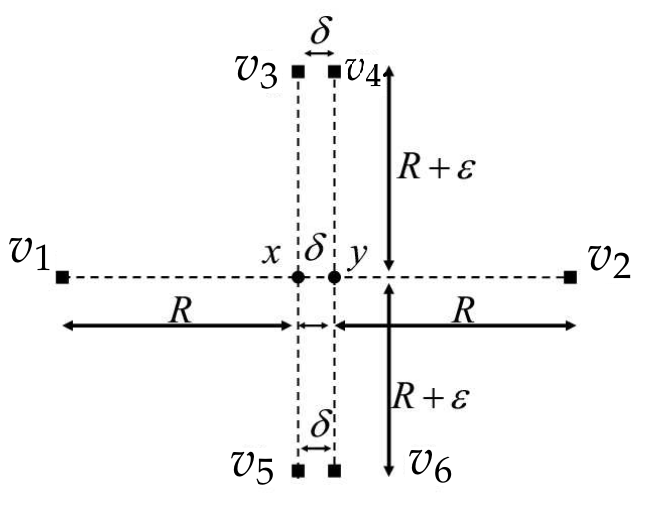
\includegraphics[scale=0.3]{imagenes/c4/Fig1}
	\caption[Ejemplo de CVQE.]{Ejemplo de CVQE. \cite{LCVQE:2007}}\label{fig:figure19}
\end{figure}

La última observación que debemos hacer está relacionada con el hecho de que la penalización por violar restricciones depende de la distancia entre los centroides implicados en ella, pero no de la distancia entre las instancias. 

\begin{observacion}
	
	El término de penalización por violar restricciones de \acs{CVQE} sólo depende de la distancia entre los centroides implicados en la restricción.
	
\end{observacion}

Para mostrar el problema que esto supone tomamos la Figura \ref{fig:figure20}, en la que se presentan dos problemas de clustering. Para ambos, los centroides existentes son $v_1$ y $v_2$, mientras que un problema incluye la restricción $ML(x_1, y)$ y el otro $ML(x_2, y)$.


\begin{figure}[!h]
	\centering
	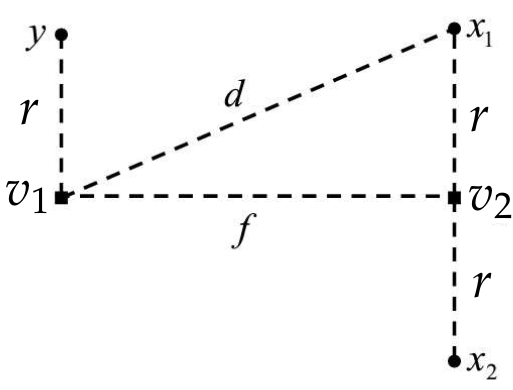
\includegraphics[scale=0.3]{imagenes/c4/Fig2}
	\caption[Ejemplo de CVQE.]{Ejemplo de CVQE. \cite{LCVQE:2007}}\label{fig:figure20}
\end{figure}

La Tabla \ref{tab:tabla3} recoge las asignaciones posibles en cada caso, así como el valor de la función $CVQE$. Vemos que, independientemente del valor de $d$ y $f$, ambos problemas tiene la misma solución, mientras que intuitivamente diríamos que violar la restricción $ML(x_1, y)$ debería acarrear una penalización mayor que violar $ML(x_2, y)$. Es más, en ambos casos la acción que aplica \acs{CVQE} es la misma, mover $v_1$ hacia $v_2$ en la recta que los une.

\begin{table}[!h]
	\centering
	\setlength{\arrayrulewidth}{1mm}
	\setlength{\tabcolsep}{10pt}
	\renewcommand{\arraystretch}{0.9}
	
	\rowcolors{2}{gray!25}{white}
	\begin{tabular}{ >{\centering\arraybackslash}m{2cm}  >{\centering\arraybackslash}m{2.5cm}>{\centering\arraybackslash}m{2cm}>{\centering\arraybackslash}m{2cm}}
		\hline
		\rowcolor{black}
		\multicolumn{4}{c}{\bf \color{white}{Valores de CVQE}}\\
		\hline
		\rowcolor{gray!50}
		\textbf{Restricción} & \textbf{$y \in c_1, x_i \in c_2$} & \textbf{$x_i,y \in c_1$} & \textbf{$x_i,y \in c_2$}  \\
		$ML(x_1, y)$ & $R^2 + R^2 + f^2$ & $R^2 + f^2 $ & $R^2 + d^2 $  \\
		$ML(x_2, y)$ & $R^2 + R^2 + f^2$ & $R^2 + f^2 $ & $R^2 + d^2 $  \\
		\hline
		
	\end{tabular}
	\caption[Valores de CVQE para el ejemplo]{Valores de CVQE para el ejemplo \cite{CECM:2012}}
	\label{tab:tabla3}
\end{table}

\subsection{El algoritmo LCVQE}

El algoritmo \acs{LCVQE} minimiza una función similar a la que minimiza \acs{CVQE}. Con la diferencia de que, para cada asignación, \acs{LCVQE} considera, como mucho, los dos clusters más naturalmente apropiados para la asignación. Por ello, la complejidad del algoritmo es independiente de $K$, al contrario de lo que sucedía en \acs{CVQE}.

Intuitivamente, las restricciones \acs{ML} violadas modifican la actualización de los centroides para desplazarlos hacia la instancia opuesta. Para las restricciones \acs{CL} violadas, se determina cuál es la instancia más lejana al centroide común, sirviendo ésta como guía para mover el segundo centroide más cercano hacia ella. Con esto tenemos que, en \acs{LCVQE}, las restricciones son simétricas, es decir, no es relevante el orden en el que se especifiquen las instancias implicadas en ellas.

\begin{observacion}
	
	En \acs{LCVQE} las restricciones son simétricas, esto es, el orden en el que se especifiquen las instancias en ellas no es relevante.
	
\end{observacion}

Para formalizar la regla de actualización es necesario definir nuevas funciones. $L_j(i)$ devuelve la instancia de entre $x_1(i)$ y $x_2(i)$ que más lejos se encuentre del centroide $v_j$. $MM(x)$ devuelve el centroide más cercano a $x$ distinto de $v_{M(x)}$. Con esto la regla de actualización queda definida como:

\begin{equation}
\begin{split}
v_j &= \frac{1}{N_j} \left[ \sum_{x_i \in c_j} x_i + 
\frac{1}{2} S_1 + \frac{1}{2} S_2 + S_3 \right]\\
S_1 &= \sum_{l=1,g(l) = j}^{ml} vl(l) \cdot x_2(l) \\
S_2 &= \sum_{l=1,g^\prime(l) = j}^{ml} vl(l) \cdot x_1(l) \\
S_3 &= \sum_{l=ml+1, j = MM(L_{M(x_1(l))}(l))}^{ml + cl} vl(l) \cdot L_{M(x_1(l))}(l)
\end{split}
\label{eqn38}
\end{equation}

donde $N_j$ en este caso se calcula como:

\begin{equation}
\begin{split}
N_j = & |c_j| + \frac{1}{2} \sum_{l=1,g(l) = j}^{ml} vl(l) + 
\frac{1}{2} \sum_{l=1,g^\prime (l) = j}^{ml} vl(l) + \\
& \sum_{l=ml+1,j = MM(L_{M(x_1(l))}(l))}^{ml + cl} vl(l)
\end{split}
\label{eqn41}
\end{equation}

Esta regla de actualización minimiza la función de error:

\begin{equation}
\begin{split}
E_j = & \frac{1}{2} \sum_{x_i \in c_j} T_{j,1} + 
\frac{1}{2} \sum_{l=1,g(l) = j}^{ml} T_{j,2} + 
\frac{1}{2} \sum_{l=ml + 1,g^\prime(l) = j}^{ml} T_{j,3} + \\
&\frac{1}{2} \sum_{l=ml+1,j = MM(L_{M(x_1(l))}(l))}^{ml + cl} T_{j,4}
\end{split}
\label{eqn42}
\end{equation}

quedando definidos los términos $T$ como:

\begin{equation}
\begin{split}
T_{j,1} &= (v_j - x_i)^2\\
T_{j,2} &= \left[ \frac{1}{2} (v_j - x_2(l))^2 \cdot vl(l) \right]\\
T_{j,3} &= \left[ \frac{1}{2} (v_j - x_1(l))^2 \cdot vl(l) \right]\\
T_{j,4} &= \left[ (v_j - L_{M(x_1(l))}(l))^2 \cdot vl(l) \right]
\end{split}
\label{eqn43}
\end{equation}

El Algoritmo \ref{alg:lcvqe} recoge de manera resumida el proceso que sigue \acs{LCVQE} para obtener una partición de los datos. 

El criterio de convergencia puede estar basado en la diferencia de los centroides entre iteraciones sucesivas, así como en criterios de asignación de instancias a clusters o evaluaciones totales de la función de error.

El algoritmo \acs{LCVQE} requiere $\mathcal{O}(p)$ operaciones en cada paso, siendo $p$ el número de dimensiones, ya que sólo se consideran tres posibles asignaciones, independientemente del valor de $K$. Por tanto \acs{LCVQE} supera en eficiencia a \acs{CVQE}, que era altamente sensible al número de clusters y de restricciones.

\begin{observacion}
	
	El algoritmo \acs{LCVQE} es computacionalmente más eficiente que \acs{CVQE}, pues en cada paso realiza $\mathcal{O}(p)$ operaciones.
	
\end{observacion}

Finalmente, podemos estudiar como se comporta el algoritmo frente al ejemplo de la Figura \ref{fig:figure20}. La Tabla \ref{tab:tabla4} muestra las asignaciones posibles en cada caso, así como los valores \acs{LCVQE}. En ambos problemas asumimos que la asignación es $x_i \in c_2$ e $y \in c_1$. En el caso de la restricción $(x_1, y)$ el centroide se actualiza según la regla $c_1 = (y + \frac{1}{2}x_1)/1.5$, y en el caso de $(x_1, y)$ tenemos que $c_1 = (y + \frac{1}{2}x_2)/1.5$, resultados intuitivamente mejores que los que obteníamos con \acs{CVQE}, ya que el centroide se mueve hacia la distancia media de las instancias en lugar de hacia el otro centroide $c_2$.

\begin{observacion}
	
	El término de penalización por violar restricciones de \acs{CVQE} involucra las características espaciales de las instancias implicadas en ella.
	
\end{observacion}

\begin{table}[!h]
	\centering
	\setlength{\arrayrulewidth}{1mm}
	\setlength{\tabcolsep}{10pt}
	\renewcommand{\arraystretch}{1}
	
	\rowcolors{2}{gray!25}{white}
	\begin{tabular}{ >{\centering\arraybackslash}m{2cm}  >{\centering\arraybackslash}m{2.5cm}>{\centering\arraybackslash}m{2cm}>{\centering\arraybackslash}m{2cm}}
		\hline
		\rowcolor{black}
		\multicolumn{4}{c}{\bf \color{white}{Valores de LCVQE}}\\
		\hline
		\rowcolor{gray!50}
		\textbf{Restricción} & \textbf{$y \in c_1, x_i \in c_2$} & \textbf{$x_i,y \in c_1$} & \textbf{$x_i,y \in c_2$}  \\
		$ML(x_1, y)$ & $(d^2 + d^2)/2$ & $d^2$ & $d^2$  \\
		$ML(x_2, y)$  & $(d^2 + d^2)/2$ & $d^2$ & $d^2$ \\
		\hline
		
	\end{tabular}
	\caption[Valores de LCVQE para el ejemplo]{Valores de LCVQE para el ejemplo \cite{CECM:2012}}
	\label{tab:tabla4}
\end{table}

\begin{algorithm}
	
	\BlankLine
	\KwIn{Conjunto de datos $X$, conjunto de restricciones $R$, centroides iniciales $V$, número de clusters $K$}
	\KwOut{Partición $P$ del conjunto de datos $X$, centroides $V$}
	\BlankLine
	\textbf{función} LCVQE($X$, $R$, $K$) \Begin{
		\BlankLine
		1. Inicialización de $GMLV_j = GCLV_j = \emptyset \;\; \forall j \in \{1, \cdots, K\}$\\
		2. Inicialización de $C$ por la regla del centroide más cercano.\\
		3. Para cada $\{(x_1(i), x_2(i))\} \in ML$ siendo $v_j$ el centroide más cercano a $x_1(i)$ y $v_n$ el centroide más cercano a $x_2(i)$ calcular:\\
		\begin{enumerate}[(a)]
			\item $\frac{1}{2} \left[(x_1(l) - v_j)^2 + (x_2(l) - v_n)^2\right] + \frac{1}{4} \left[(x_1(l) - v_n)^2 + (x_2(l) - v_j)^2\right]$
			
			\item $\frac{1}{2}(x_1(l) - v_j)^2 + \frac{1}{2}(x_2(l) - v_j)^2$
			
			\item $\frac{1}{2}(x_1(l) - v_n)^2 + \frac{1}{2}(x_2(l) - v_n)^2$
		\end{enumerate}
		Si (a) es minimal $\rightarrow$ $GMLV_j = GMLV_j \cup x_2(l)$ y $GMLV_n = GMLV_n \cup x_1(l)$. Asignar $x_1$ a $c_j$ y $x_2$ a $c_n$. \\ Si (b) es minimal $\rightarrow$ asignar $x_1$ y $x_2$ a $c_j$. \\ Si (c) es minimal $\rightarrow$ asignar $x_1$ y $x_2$ a $c_n$.\\
		
		4. Para cada $\{(x_1(i), x_2(i))\} \in CL$ con $v_j$ el centroide más cercano a $x_1(i)$ y $v_n$ el centroide más cercano a $x_2(i)$, y siendo $Max_n(l) = argmax_{x_i(l)}(x_i(l)- v_n)^2$. Tomamos $j$ como el centroide más cercano a $Max_n(l)$ que no sea $n$ y calculamos:
		\begin{enumerate}[(a)]
			\item $\frac{1}{2} (x_1(l) - v_j)^2 + \frac{1}{2}(x_2(l) - v_j)^2 + \frac{1}{2} (Max_n(l) - v_{MM(Max_j(l))})^2$
			
			\item $\frac{1}{2}\left[(x_1(l) - v_j)^2 + (x_2(l) - v_n)^2\right]$
		\end{enumerate}
		Si (a) es minimal $\rightarrow$ $GCLV_{MM(Max_j(l))} = GCLV_{MM(Max_j(l))} \cup Max_j(l)$ y asignar $x_1$ y $x_2$ a $c_j$. \\ Si (b) es minimal $\rightarrow$ Asignar $x_1$ a $c_j$ y $x_2$ a $c_n$.\\
		5. Actualizar cada centroide $v_j$ en $V$ como sigue: 
		$ v_j = \frac{1}{N_j}\left[Sum(c_j) + \frac{1}{2}Sum(GMLV_l) + Sum(GCLV_j)\right]$\\
		6. Iterar entre (2.) y (5.) hasta converger\\
		7. \KwRet $C$, $V$
		\BlankLine
	}
	\caption{\acf{LCVQE}}
	\label{alg:lcvqe}
\end{algorithm}






\section{Relational Dirichlet Process - Means (RDP - Means)} \label{rdpmYtvc}

Tomamos como referencia principal el trabajo de Daniel Khashabi et al. (2015) \cite{RDPM:2015}. En él, los autores incorporan las restricciones desde una perspectiva distinta a las anteriores. Así, modelan el conjunto de instancias y el conjunto de restricciones de manera diferente; es por ello que llaman \acf{TVClust} al método base para \acf{RDPM}.

Para ser más específicos, \acs{TVClust} combina una mezcla de Procesos de Dirichlet, aplicados sobre el conjunto de instancias, y una interpretación del conjunto de restricciones que las considera como un grafo aleatorio. Además, los autores derivan este modelo, basándose en el algoritmo \acf{DPM} \cite{DPM:2012} combinado con el modelo de las restricciones, para obtener un algoritmo determinista que incorpora las mismas a \acs{DPM}, esto es, el algoritmo \acf{RDPM}.

\subsection{El modelo Bayesiano no paramétrico}

Introducimos las particularidades relacionadas con el modelo de datos sobre el que aplicaremos clustering. El conjunto de instancias $X$ viene definido tal y como se especifica al inicio de la Sección \ref{ch:Algoritmos}, y el conjunto de restricciones $R$ como una matriz simétrica de $n \times n$. En $R$ se encuentran almacenadas todas las posibles restricciones que involucran a parejas de instancias. Así, tomando $x_i$ y $x_j$ como dos instancias, basta con obtener el valor $R_{i,j}$ en la matriz para saber la relación que existe entre ellas. Si $R_{i,j} = 1$, entonces existe una restricción de tipo \acf{ML} entre $x_i$ y $x_j$, si $R_{i,j} = 0$ la restricción será de tipo \acf{CL}, y no existirá relación entre las instancias en cualquier otro caso.

Consideramos los dos conjuntos de datos de los que disponemos, $X$ y $R$, como dos formas distintas de ver la estructura de clusters subyacente. Cabe destacar que cualquiera de estas dos estructuras es suficiente para llevar a cabo procesos de clustering clásicos, ya sean métodos como \acf{KM} (Sección \ref{ap:kmeans}), en el caso de $X$, o \textit{normalized graph-cut} en el caso de $R$.

La aproximación mediante \acs{TVClust} consiste en agregar información de los dos modelos mediante un enfoque Bayesiano, de manera que sea posible alcanzar un consenso entre ambos, que tenga como resultado la partición de $X$. Dada la estructura de clustering latente, que se supone común, los datos de ambas interpretaciones se modelan mediante dos procesos generativos distintos: $X$ se modela mediante Mezcla de Procesos de Dirichlet, y $R$ mediante un grafo aleatorio.

Considerar modelos distintos para entender los datos y las restricciones es de especial utilidad cuando ninguno de los dos puede ser tomado como completamente fiable. Mientras que otros métodos de clustering como COP-K-medias (Sección \ref{copkm}) confían en la exactitud de las restricciones, \acs{TVClust} hace una interpretación relajada de las mismas, haciéndolo más robusto ante errores. Podría decirse que, en \acs{TVClust}, $R_{i,j} = 1$ equivale una una restricción \textit{May-Link}, mientras que $R_{i,j} = 0$ se asociaría a una \textit{May-Not-Link}, en contraste con las ya conocidas \acf{ML} y \acf{CL}.

\subsubsection{Modelo para las instancias}

Como ya hemos visto, utilizamos una Mezcla de Procesos de Dirichlet como modelo de clustering subyacente para el conjunto de datos $X$. Tomamos $\theta_i$ como el parámetro del modelo asociado
a la instancia $x_i$, que es modelado como una muestra independiente e idénticamente distribuida \footnote{\textbf{iid} es la abreviatura en inglés para ``independiente e idénticamente distribuida''.} de una distribución aleatoria $G$, que se obtiene en base a un Proceso de Dirichlet $\mathsf{DP}(\alpha, G_0)$:

\begin{equation}
\{\theta_0, \cdots, \theta_n\} \;\; t.q. \;\; G \overset{iid}{\thicksim} G, \;\;\; G \thicksim \mathsf{DP}(\alpha, G_0)
\label{eqn44}
\end{equation}

Con esto, conociendo la distribución de $\theta_{\backslash i}$ definida como $\theta_{\backslash i} = \{\theta_0, \cdots, \theta_{i-1},\theta_{i+1}, \cdots,\theta_n\}$ podemos conocer la de $\theta_{i}$ aplicando el esquema de Balckwell-MacQueen \cite{Blackwell:1973}:

\begin{equation}
p(\theta_{i}|\theta_{\backslash i}) \varpropto \sum_{k = 1}^{K} n_{-i,k} \delta_{\theta_{k}^*}(\theta_{i}) + \alpha G_0(\theta_{i})
\label{eqn45}
\end{equation}

donde asumimos que existen $K$ \footnote{La interpretación de $K$ en esta sección es distinta a la propuesta al inicio de la Sección \ref{ch:Algoritmos}, en la introducción a la notación.} valores únicos entre $\theta_{\backslash i}$ notados como $\{\theta_{1}^*, \cdots, \theta_{K}^*\}$, $\delta_{\theta_{k}^*}(\cdot)$ es la función delta de Kronecker, y $n_{-i,k}$ es el número de instancias agrupadas en el cluster $c_k$ excluyendo la instancia $i$. Así, la Ecuación \ref{eqn45} puede entenderse dentro de los métodos de clustering tradicionales en el sentido de que con una probabilidad positiva, $\theta_i$ tomará uno de los valores del conjunto $\{\theta_{1}^*, \cdots, \theta_{K}^*\}$, esto es, la instancia asociada se incluirá en uno de los clusters presentes. Para simplificar este concepto podemos emplear la Metáfora del Restaurante Chino, propuesta por Aldous (1983), en la que asignar $\theta_i$ a un cluster es análogo a sentar un cliente en una mesa del restaurante. El cliente puede sentarse en una mesa ya ocupada o en una que estaba vacía.

Dado $\theta_i$, utilizamos una familia de funciones paramétricas $p(x_i|\theta_i)$ para modelar la instancia $x_i$, en concreto tomaremos las familia de las exponenciales:

\begin{equation}
p(x|\theta) = exp(\langle T(x), \theta \rangle - \psi(\theta) - h(x))
\label{eqn46}
\end{equation}

donde $\psi(\theta)$ es la función \textit{log-partition} para la familia exponencial $\psi(\theta) = log \int exp(\langle x, \theta \rangle - h(x))dx$, y $T(x)$ es el vector de estimadores suficientes de la distribución de probabilidad. En el caso de la familia exponencial la dimensión del vector de estimadores suficientes es igual al número de parámetros estimables. Por simplicidad asumimos que $x$ es el vector de estimadores suficientes aumentado y obtenemos:

\begin{equation}
p(x|\theta) = exp(\langle x, \theta \rangle - \psi(\theta) - h(x))
\label{eqn47}
\end{equation}

Con esta formulación definimos:

\begin{equation}
\begin{split}
\mathbb{E}_p[x] &= \nabla_{\theta} \psi(\theta) \\
Cov_p[x] &= \nabla_{\theta}^2 \psi(\theta)
\end{split}
\label{eqn48}
\end{equation}

Y por conveniencia escogeremos la medida base para $G_0$ en $\mathsf{DP}(\alpha, G_0)$ de entre la familia de conjugados, que toma la siguiente forma:

\begin{equation}
d G_0(\theta| \tau, \eta) = exp(\langle \theta, \tau \rangle - \eta\psi(\theta) - m(\tau, \eta))
\label{eqn49}
\end{equation}

donde $\tau$ y $\eta$ son parámetros de la distribución base. Dadas estas definiciones de probabilidad y conjugado, la posterior distribución sobre $\theta$ será la familia exponencial de la misma forma que la inicial, pero escalando los parámetros a $\tau + x$ y $\eta + 1$ (para más detalles consultar \cite{RDPM:2015}).

La familia exponencial contiene multitud de distribuciones empleadas en la práctica. Por ejemplo, las distribuciones Gaussianas se utilizan para modelar valores reales en un espacio $\mathbb{R}^p$. 

\subsubsection{Modelo para las restricciones}

Dado $\theta_{1:n} = \{\theta_1, \cdots \theta_n\}$ podemos resumir las estructura del clustering mediante una matriz $H$ con dimensiones $n\times n$, donde $H_{i,j} = \delta_{\theta_i}(\theta_j)$. Cabe destacar que la matriz $H$ es distinta a la matriz $R$, ya que esta última representa las restricciones y puede ser entendida como una muestra aleatoria de la estructura de clustering contenida en $H$. Con esto, el objetivo es inferir $H$ en base a $R$.

Modelamos $R$ mediante el siguiente proceso generativo: con probabilidad $p$, una arista existente en el grafo descrito por $H$ se conserva en $R$, y con probabilidad $q$, una falsa arista de $H$ se añade a $R$. Por ejemplo, tomando $(i,j) \in \{1, \cdots, n\}$:

\begin{equation}
\begin{cases}
p(R_{i,j} = 0 | H_{i,j} = 1) = p\\
p(R_{i,j} = 1 | H_{i,j} = 0) = 1 - p\\
p(R_{i,j} = 0 | H_{i,j} = 0) = q\\
p(R_{i,j} = 1 | H_{i,j} = 0) = 1 - q
\end{cases}
\label{eqn50}
\end{equation}

Dicho de otra forma, los parámetros $p$ y $q$ representan la credibilidad de los valores presentes en la matriz $R$, mientras que $1 - p$ y $1 - q$ representan la probabilidad de error. El valor concreto que se debe asignar a $p$ y $q$ varía para cada problema; pueden ser obtenidos mediante conocimiento experto o con técnicas de aprendizaje desde datos.

\subsubsection{Inferencia mediante muestreo de Gibbs}

Es posible derivar un esquema de muestro de Gibbs para el modelo de \acs{TVClust}, que en esencia es similar al que emplea \acf{DPM}. La distribución de muestreo que emplearemos viene definida por:

\begin{equation}
\begin{split}
p(\theta_i | \theta_{\backslash i}, & x_i, R, p, q) \varpropto \\
 &\sum_{k = 1}^{K} n_{-i,k} p(x_i|\theta_{k}^*) \delta_{\theta_{k}^*}(\theta_{i}) \left(\frac{p}{1-q}\right)^{f_{k}^i} \left(\frac{1-p}{q}\right)^{s_{k}^i} + \alpha p_{G_0}(x_i)p_{G_0}(\theta_i | x_i)
\end{split}
\label{eqn51}
\end{equation}

donde 

\begin{equation}
\begin{cases}
f_{k}^i = \#\{j:\theta_j = \theta_{k}^*, R_{i,j} = 1\}\\
s_{k}^i = \#\{j:\theta_j = \theta_{k}^*, R_{i,j} = 0\}\\
\end{cases}
\label{eqn52}
\end{equation}

El proceso de cálculo y simplificación que deriva en estas ecuaciones se encuentra detallado en el trabajo de Daniel Khashabi et al. (2015) \cite{RDPM:2015}.

Retomando la analogía del restaurante chino, podemos interpretar la distribución de muestreo de $\theta_i$ de la siguiente manera: si la instancia $i$ es \textit{amiga} de la instancia $j$, entonces $R_{i,j} = 1$, por otra parte, si dos instancias son \textit{desconocidas} entonces $R_{i,j} = 0$. Con esto, podemos interpretar el valor $f_{i}^k$ como el número de amigos de la instancia $i$ en la mesa $k$, y $s_{i}^k$ como el número de desconocidos.

Tal y como hemos visto, los valores $p$ y $q$ representan la credibilidad de las restricciones, esto es, el nivel de confianza en que son correctas. Para representar un grado de confianza alto generalmente estableceremos que $p > 1 - q$. Con esto, y tomando en consideración la Ecuación \ref{eqn51}, la probabilidad de que una persona sea asignada a una mesa no sólo aumenta con la popularidad de la misma, sino que también lo hace con el número de amigos de la instancia en la mesa ($f_{i}^k$) y disminuye con el número de desconocidos ($s_{i}^k$).

Una mejora aplicable al modelo consiste en modificar la regla de actualización del conjunto de parámetros $ \{\theta_1, \cdots, \theta_n\}$, de manera que, en lugar de actualizar los parámetros particulares de cada instancia de manera secuencial, se actualiza un conjunto de parámetros asociados a los clusters $\{\theta_i^*, \cdots, \theta_K^*\}$, así como los indicadores de asignación de instancias a clusters (las etiquetas) $\{z_i, \cdots, z_n\}$ donde $z_i\in \{1, \cdots, K\}$ indica el cluster al que esta asignado la instancia $i$. Entonces la nueva regla de actualización es:

\begin{equation}
\begin{cases}
p(z_i = k) \varpropto n_{-i,k}p(x_i,\theta_k^*)\left(\frac{p}{1-q}\right)^{f_{k}^i} \left(\frac{1-p}{q}\right)^{s_{k}^i} \\
p(z_i = k_{nuevo}) \varpropto \alpha \int p(x_i,\theta_k^*)dG_0
\end{cases}
\label{eqn53}
\end{equation}

\subsection{Reparametrización de la familia exponencial para RDP-means}

Para comprender \acf{RDPM} es necesario introducir el concepto de divergencia de Bregman, así como su relación con la familia de funciones exponenciales. Comenzamos con la definición formal de la divergencia de Bregman:

\begin{definicion}
	
	\textbf{Divergencia de Bregman (1967)}: Definida una función estrictamente convexa $\phi: \mathcal{S} \rightarrow \mathbb{R}$, de forma que el dominio $\mathcal{S} \subseteq \mathbb{R}^p$ es un conjunto convexo, y $\phi$ es diferenciable en $ri(\mathcal{S})$, siendo este el interior relativo de $\mathcal{S}$ donde su gradiente $\nabla \phi$ existe. Dados dos puntos $x,y \in \mathbb{R}^p$, la divergencia de Bregman $D_{\phi}(x,y): \mathcal{S} \times ri(\mathcal{S}) \rightarrow [0, + \infty)$ viene definida como: \cite{RDPM:2015}
	
	$$ D_{\phi}(x,y) = \phi(x) - \phi(y) - \langle x - y, \nabla \phi(y)  \rangle $$
	
\end{definicion}

La divergencia de Bregman es una clase general de medidas de distancia, por ejemplo, tomando $\phi$ como una función cuadrática, la divergencia de Bregman es equivalente a la distancia Euclídea \cite{Banerjee:2005}.

Existe una aplicación biyectiva entre la familia exponencial y las divergencias de Bregman, tal y como demostraron Foster y Warmuth (2002) \cite{Forster:2002}. Dada esta conexión, Banerjee et al. (2005) \cite{Banerjee:2005} construyeron un algoritmo en base a \acf{KM} que utiliza la divergencia de Bregman como medida de distancia, en lugar de la distancia Euclídea.

\begin{definicion}
	
	\textbf{El Conjugado de Legendre}: Para una función $\psi(\cdot)$ definida sobre el dominio $\mathbb{R}^p$, se define como su conjugado convexo $\psi^*(\cdot)$ como $\psi^*(\mu) = sum_{\theta \in dom(\phi)}\{\langle \mu, \theta \rangle - \psi(\theta) \}$. Además, si la función $\psi(\theta)$ es cerrada y convexa, entonces $(\psi^*)^* = \psi$. \cite{RDPM:2015}
	
\end{definicion}


Se puede demostrar que la función \textit{log-partition} de la familia exponencial es una función cerrada y convexa. Por tanto, existe una biyección entre el parámetro $\mu$ del conjugado de Legendre $\psi^*(\cdot)$, y el parámetro de la familia exponencial, $\theta$, en la función \textit{log-partition} definida para la familia exponencial en la Ecuación \ref{eqn46}. Con esto, podemos reescribir la probabilidad definida por la Ecuación \ref{eqn47} usando la divergencia de Bregman y el conjugado de Legendre:

\begin{equation}
p(x|\theta) = p(x|\mu) = exp(-D_{\psi^*}(x, \mu)) f_{\psi^*}(x)
\label{eqn54}
\end{equation}

donde $f_{\psi^*}(x) = exp(\psi^*(x) - h(x))$. Una consecuencia de esta nueva parametrización es que la probabilidad asociada a cualquier instancia $x$ está relacionada con cómo de \textit{lejos} está la misma del cluster parametrizado con $\mu$, midiendo la distancia según la divergencia de Bregman $D_{\psi^*}(x, \mu)$.

De manera similar podemos reescribir la Ecuación \ref{eqn49} en términos de la divergencia de Bregman y el conjugado de Legendre:

\begin{equation}
p(\theta|\tau, \eta) = p(\mu|\tau, \eta) = exp \left(-\eta D_{\psi^*}(\frac{\tau}{\eta}, \mu)\right) g_{\psi^*}(\tau, \eta)
\label{eqn55}
\end{equation}

donde $g_{\psi^*}(\tau, \eta) = exp(\eta \psi(\theta) - m(\tau, \eta))$

\subsection{Escalando las distribuciones para RDP-means}

\begin{lema}

	\textbf{Jiang et al (2012)} \cite{DPM:2012}: Dada la familia exponencial definida en la Ecuación \ref{eqn46}, definimos otra distribución de probabilidad con parámetro $\widetilde{\theta}$ y la función \textit{log-partition} $\widetilde{\psi}(\cdot)$, donde $\widetilde{\theta} = \gamma\theta$ y $\widetilde{\psi}(\widetilde{\theta}) = \gamma \psi (\widetilde{\theta}/\gamma)$, entonces:
	
	\begin{enumerate}
		
		\item La distribución de probabilidad escalada $\widetilde{p}(\cdot)$ definida con parámetro $\widetilde{\theta}$ y función \textit{log-partition} $\widetilde{\psi}(\cdot)$, es una distribución de probabilidad propia que pertenece a la familia exponencial.
		
		\item La media y la varianza de la distribución de probabilidad $\widetilde{p}(\cdot)$ son:
		
		$$ \mathbb{E}_{\widetilde{p}}(x) = \mathbb{E}_{p}(x), \;\;\;\; Cov_{\widetilde{p}}(x) = \frac{1}{\gamma}Cov_p(X) $$
		
		\item El conjugado de Legendre de $\widetilde{\psi}(\cdot)$ es $\widetilde{\psi}^*(\widetilde{\theta}) = \gamma \psi^*(\widetilde{\theta}) $
		
	\end{enumerate}
	\label{lema:1}
\end{lema}

El resultado más importante derivado del Lema \ref{lema:1} es que la covarianza $Cov_p(x)$ escala con $1/\gamma$, que tiende a $0$ para valores grandes de $\gamma$, mientras que la media $\mathbb{E}_{p}(x)$ se mantiene invariante. Por tanto podemos obtener un algoritmo determinista cuando $\gamma$ tiende a infinito.

Con esto, las Ecuaciones \ref{eqn54} y \ref{eqn55} pueden ser escritas como:

\begin{equation}
\begin{split}
&\widetilde{p}(x|\theta, \gamma) = \widetilde{p}(x|\mu, \gamma) = exp(-\gamma D_{\psi^*}(x,\mu)) f_{\gamma \psi^*}(x)\\
&\widetilde{p}(\theta|\tau,\eta,\gamma) = \widetilde{p}(\widetilde{\mu}|\tau,\eta,\gamma) = exp\left(-\eta D_{\psi^*}(\frac{\tau}{\eta}, \mu)\right)g_{\gamma \psi^*}(\tau / \gamma, \eta / \gamma)
\end{split}
\label{eqn56}
\end{equation}

\subsection{Asintóticos de TVClust}

Usando la distribución escalada definida en la Ecuación \ref{eqn56} podemos reescribir la regla de actualización de Gibbs descrita en la Ecuación \ref{eqn53} como sigue:

\begin{equation}
\begin{cases}
p(z_i = k) \varpropto n_{-i,k}exp(-\gamma D_{\psi^*}(x_i,\mu_k))\left(\frac{p}{1-q}\right)^{f_{k}^i} \left(\frac{1-p}{q}\right)^{s_{k}^i} \\
p(z_i = k_{nuevo}) \varpropto \alpha \int \widetilde{p}(x_i|\theta)\widetilde{p}(\theta|\tau, \eta)d\theta
\end{cases}
\label{eqn57}
\end{equation}

Siguiendo el proceso de cálculo y simplificación detallado en el trabajo de Daniel Khashabi et al. (2015) \cite{RDPM:2015}, podemos transformar la Ecuación \ref{eqn57} en:

\begin{equation}
\begin{cases}
p(z_i = k) \varpropto n_{-i,k}exp(-\gamma D_{\psi^*}(x_i,\mu_k)) - \xi_1 f_{k}^i + \xi_2 s_{k}^i \\
p(z_i = k_{nuevo}) \varpropto \nu(x_i; \tau, \eta, \gamma) exp(-\gamma \lambda)
\end{cases}
\label{eqn58}
\end{equation}

Donde $\xi_1 = ln\left(\frac{p}{1-q}\right)$ y $\xi_2 = ln\left(\frac{q}{1-p}\right)$, esto es, $\xi_1$ y $\xi_2$ representan, respectivamente, la probabilidad de que exista o no exista una restricción.

Cuando $\gamma$ tiende a infinito, el muestreador de Gibbs deriva en un algoritmo determinista, en el que, en cada iteración, la asignación de $x_i$ a un cluster se determina comparando los $K+1$ valores descritos por:

\begin{equation}
\{D_{\psi*}(x_i, \mu_1) - \xi_1 f_{1}^i  + \xi_2 s_{1}^i, \cdots, D_{\psi*}(x_i, \mu_K) - \xi_1 f_{K}^i + \xi_2 s_{K}^i, \;\; \lambda \}
\label{eqn59}
\end{equation}

Si el valor k-ésimo (con $k = 1, \cdots, K$) es el más pequeño, entonces $x_i$ se asigna al cluster k-ésimo, por el contrario, si $\lambda$ es el menor valor, se crea un cluster nuevo con $x_i$ como única instancia asignada.

\subsection{Muestreo de los parámetros de los clusters}

Daniel Khashabi et al. (2015) \cite{RDPM:2015} demuestran que la función que muestrea los parámetros para los clusters es equivalente a una media de las instancias que éstos contienen bajo las condiciones adecuadas, esto es, tomando $\gamma \rightarrow \infty$ y argumentos iguales para la divergencia de Bregman. De esta manera, la ecuación de actualización de los parámetros para los clusters es:

\begin{equation}
\mu_k = \frac{1}{n_k} \sum_{i:z_i = k} x_i
\label{eqn61}
\end{equation}

Esto completa el algoritmo \acf{RDPM}; podemos resumir el proceso de cálculo que éste lleva a cabo en el Algoritmo \ref{alg:rdpm}:

\subsection{Función objetivo de RDP-means}

\begin{teorema}
	
	El algoritmo de clustering con restricciones RDP-means minimiza de manera iterativa la siguiente función:
	
	\begin{equation}
	min_{\{\mathcal{L}_k\}_{k=1}^K} \sum_{k=1}^{K} \sum_{i \in \mathcal{L}_k} \left[D_{\phi}(x_i, \mu_k) - \xi_1 f_{k}^i  + \xi_2 s_{k}^i\right] + \lambda K
	\label{eqn60}
	\end{equation}
	
	donde $\{\mathcal{L}_1, \cdots, \mathcal{L}_k\}$ representan una partición de las $n$ instancias.
	
\end{teorema}

\subsection{Efectos de los cambios sobre $\xi_1$ y $\xi_2$}

Tomando $\xi_1, \xi_2 \rightarrow 0$, el algoritmo \acs{RDPM} se comporta de manera idéntica a \acs{DPM}, esto es, no se tiene en consideración la información proporcionada por las restricciones. Por otra parte, si $\xi_1, \xi_2 \rightarrow \infty$ se pone todo el peso en las restricciones y no se consideran las instancias para el proceso de clustering; en otras palabras, el conjunto de cluster se genera de acuerdo a la matriz $R$ únicamente. De manera similar, podemos escoger poner más peso en las restricciones \textit{may-link} sobre las \textit{may-not-link} estableciendo $\xi_1 > \xi_2$ y viceversa.

A pesar del control que $\xi_1$ y $\xi_2$ permiten sobre el proceso de clustering, la función objetivo de \acs{RDPM} (Ecuación \ref{eqn60}) posee un gran número de mínimos locales y, dado que el algoritmo la minimiza con un proceso \textit{greedy}, corremos el riesgo de caer en un mínimo local. Los autores Daniel Khashabi et al. (2015) \cite{RDPM:2015} muestran experimentalmente que establecer $\xi_1 = \xi_2 = \xi$, con un valor pequeño para $\xi_0$, que se incrementará con el paso de las iteraciones en función de un ratio dado, proporciona mejores resultados que un esquema de libre configuración para $\xi_1$ y $\xi_2$.

\begin{algorithm}
	\KwIn{Conjunto de datos $X$, matriz de restricciones $R$, parámetro de la divergencia de Bregman $\psi*$, los parámetros $\lambda$, $\xi_0$, y el ratio de incremento $\xi_{rate}$}
	\BlankLine
	\KwOut{La asignación $z = [z_1, z_1, \cdots, z_n]$}
	\BlankLine
	\textbf{función} RDPM($X$, $R$, $\psi*$, $\lambda$, $\xi_0$, $\xi_{rate}$) \Begin{
		\BlankLine
		
		1. Inicializar $\xi \leftarrow \xi_0$ y asignar todas las instancias a un mismo cluster\\
		2. Iterar hasta converger como sigue:\\
		\While{$no \;\; convergencia$}{
			
			\For{$x_i \in X$}{
				
				\For{$\mu_k \in C$}{
					
					Calcular los valores $f_{k}^i$ y $s_{k}^i$ a partir de $R$.\\
					$dist(x_i, \mu_k) \leftarrow D_{\psi*}(x_i, \mu_k) - f_{k}^i \xi_1 + \xi_2 s_{k}^i$
				
				}
				\texttt{//$d_{min}$ es la distancia minima e $i_{min}$ es el índice de la misma}
				$[d_{min}, i_{min}] \leftarrow \{dist(x_i, \mu_1), \cdots, dist(x_i, \mu_k)\}$
				
				\eIf{$d_{min} < \lambda$}{
					$z_i \leftarrow i_{min}$
				}{
					$C \leftarrow \{C \cup \{x_i\}\}$ \texttt{//Crear un nuevo cluster}\\
					$K \leftarrow K + 1$
				}
				
			}
			
			\For{$\mu_k \in C$}{
				\eIf{$|c_k| > 0$}{
					
					$\mu_k \leftarrow \frac{\sum_{x_i \in c_j} x_i}{|c_j|}$
					
				}{
					
					Eilimar el cluster $c_j$ y propagar los cambios
				
				}
			}
			
			$\xi \leftarrow \xi \times \xi_{rate}$
			
		}
		\BlankLine
		\KwRet $C$
	}
	\caption{\acf{RDPM}}
	\label{alg:rdpm}
\end{algorithm}

%cambiar familia de las exponenciales por familia exponencial

%Revisar que no pone distancia euclideana en ninguna parte








